\documentclass[10pt]{article}

\usepackage{graphicx}
\usepackage{ifthen}
\input{/home/donma/Documents/src/ib/AITrading_24_7/StepByStep/aitrading-preamble.tex}
\usepackage[nameinlink,capitalise]{cleveref}

\newboolean{draftmode}
\setboolean{draftmode}{false}
\input{/home/donma/Documents/Pointer/TexCompilationTools/SumCounterControl.tex}
\input{/home/donma/Documents/Pointer/TexCompilationTools/SumControl.tex}
\input{/home/donma/Documents/Pointer/TexCompilationTools/SumAuthorControl.tex}

\geometry{top=0.68in,bottom=0.68in,left=0.72in,right=0.72in}
\setstretch{1.0}
\setlength{\parskip}{0.24em}
\setlength{\parindent}{0pt}
\setlength{\headheight}{14pt}
\setcounter{tocdepth}{1}
\fancyhead[L]{\small\textcolor{uablue}{Weekly Research Update}}
\fancyhead[R]{\small\textcolor{uablue}{September 2, 2026}}
\hypersetup{
  colorlinks=true,
  linkcolor=uablue,
  urlcolor=uablue,
  citecolor=accent,
  filecolor=accent,
  menucolor=uablue,
  linktoc=all,
  breaklinks=true,
  pdftitle={Weekly Research Update for September 2, 2026},
  pdfsubject={Embedding retrieval, bi-objective revision, and stochastic multiple knapsack},
  pdfauthor={Muting Don Ma}
}

\newcommand{\statusdone}{\textcolor{definitiongreen}{\textbf{Completed:}}\ }
\newcommand{\statusprogress}{\textcolor{uablue}{\textbf{In progress:}}\ }
\newcommand{\statusblocked}{\textcolor{accent}{\textbf{Blocked:}}\ }
\newcommand{\updatehead}[2]{%
  \vspace{0.22em}\noindent\textbf{\textcolor{uablue}{#1. #2}}\par\vspace{0.04em}}
\newcommand{\projectline}[1]{%
  {\small\noindent\textbf{Name:} Muting (Don) Ma\hfill
    \textbf{Project:} #1\hfill
    \textbf{Date:} September 2, 2026\par}
  \vspace{0.18em}\hrule\vspace{0.42em}}
\newenvironment{tightitems}{%
  \begin{itemize}[leftmargin=1.15em,label=\textcolor{uablue}{\scriptsize$\bullet$},
    topsep=0.08em,itemsep=0.17em,parsep=0pt,partopsep=0pt]}{\end{itemize}}
\newcommand{\artifact}[2]{\href{#1}{#2}}

\begin{document}

\hypersetup{pageanchor=false}
\begin{titlepage}
\thispagestyle{empty}
\vspace*{0.18\textheight}
\begin{center}
  {\Huge\bfseries\textcolor{uablue}{Weekly Research Update}}\\[0.8em]
  {\Large Three Project Progress Report}\\[2.2em]
  {\large Muting (Don) Ma}\\[0.45em]
  {\large September 2, 2026}\\[3em]
  \fcolorbox{uablue}{uablue!4}{%
    \parbox{0.76\textwidth}{\centering\large
      Embedding Retrieval Capacity\\[0.6em]
      Bi-objective Trajectory Revision C1\\[0.6em]
      Stochastic Multiple Knapsack Manuscript}}
  \\[3em]
  \small Public artifacts:
  \href{https://github.com/mutingma123/OpenProjects}{OpenProjects repository}
\end{center}
\end{titlepage}
\hypersetup{pageanchor=true}

\clearpage
\pagenumbering{roman}
\setcounter{page}{1}
\tableofcontents
\clearpage

\pagenumbering{arabic}
\setcounter{page}{1}

\section{Embedding Retrieval Capacity}
\label{sec:retrieval}
\projectline{Embedding Retrieval Capacity}

\updatehead{1}{Current objective}
\sumpara The objective transfers the representation result into the proposal's decision setting. \sumparaend
\begin{tightitems}
  \item \fin Translate fixed-dimensional retrieval limits into a proposal-ready account of when representation error can undermine optimization decisions. \fine
\end{tightitems}

\updatehead{2}{Progress since the last meeting}
\sumpara The progress distinguishes completed exposition from the open proposal theorem. \sumparaend
\begin{tightitems}
  \item \fin \statusdone Built a 60-frame, 72-slide dissection with prerequisites, the full proof, experiments, and every appendix. \fine
  \item \fin \statusdone Separated the proved margin bound, the observed free-vector threshold, the LIMIT benchmark, and the architecture implications. \fine
  \item \fin \statusprogress Identified a distribution-dependent theorem that carries retrieval error into feasibility loss or operational regret as the proposal transfer. \fine
\end{tightitems}

\updatehead{3}{Key result or lesson}
\sumpara The key result states the lower bound and the empirical gap without conflating them. \sumparaend
\begin{tightitems}
  \item \fin If every size-\(k\) answer must be realized with margin \(2\gamma\), then \(d\geq \log\binom{n}{k}/\log(1+1/\gamma)\) \cite{weller2026}. \fine
  \item \fin LIMIT shows a further gap between geometric capacity and learned use of that capacity. \fine
  \item \fin The \artifact{https://github.com/mutingma123/OpenProjects/blob/main/EmbeddingRetrievalLimitations/Figures/RetrievalCapacityMap.png}{public causal map} connects both findings to decision reliability. \fine
\end{tightitems}

\begin{figure}[!ht]
  \centering
  \href{https://github.com/mutingma123/OpenProjects/blob/main/EmbeddingRetrievalLimitations/Figures/RetrievalCapacityMap.png}{%
    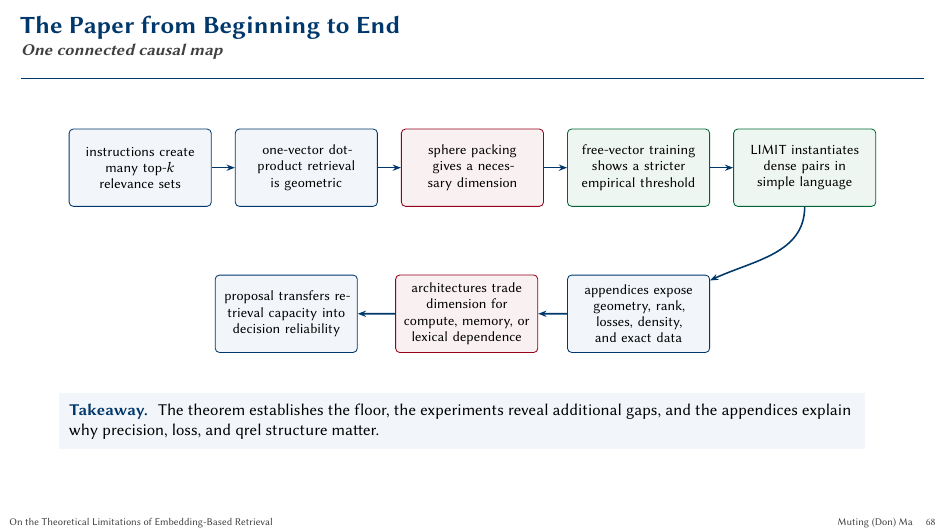
\includegraphics[width=0.58\textwidth]{../../EmbeddingRetrievalLimitations/Figures/RetrievalCapacityMap.png}}
  \caption{Evidence chain from retrieval capacity to decision reliability.}
  \label{fig:retrieval-map}
\end{figure}

\updatehead{4}{Input needed from Dr. Gong}
\sumpara The requested input fixes the theorem target and the empirical comparison. \sumparaend
\begin{tightitems}
  \item \fin Should the transfer theorem target feasibility loss, objective regret, or both? \fine
  \item \fin Should the first stress test compare single-vector retrieval with multi-vector retrieval, hybrid retrieval, or both? \fine
\end{tightitems}

\updatehead{5}{Before the next meeting}
\sumpara The deliverables move from exposition to a proposal-ready result. \sumparaend
\begin{tightitems}
  \item \fin Draft the proposal subsection. \fine
  \item \fin Formalize the first error-to-regret proposition. \fine
  \item \fin Specify a toy operational stress test and metrics. \fine
\end{tightitems}

\vspace{0.25em}
{\footnotesize\textbf{Public artifacts:}
\artifact{https://github.com/mutingma123/OpenProjects/tree/main/EmbeddingRetrievalLimitations}{project folder};
\artifact{https://github.com/mutingma123/OpenProjects/tree/main/EmbeddingRetrievalLimitations/Figures}{selected snapshot}.\par}

\clearpage
\section{Bi-objective Trajectory Revision C1}
\label{sec:biobj}
\projectline{Bi-objective Trajectory Revision C1}

\updatehead{1}{Current objective}
\sumpara The objective closes the mathematical repair and the remaining evidence chain. \sumparaend
\begin{tightitems}
  \item \fin Close revision C1 by making pair-pass uncertainty auditable as expected collision cost and completing the validation and comparison sequence. \fine
\end{tightitems}

\updatehead{2}{Progress since the last meeting}
\sumpara The progress reports the two diverged branches and their present closure status. \sumparaend
\begin{tightitems}
  \item \fin \statusdone The \texttt{revision/c1} branch derived the Rayleigh survival map and least-gap nested-event result, then removed the retired shared-cell average and count detour. \fine
  \item \fin \statusdone The revised estimand regenerated schedule costs, the control menu, break-even results, figures, and the evidence boundary. \fine
  \item \fin \statusprogress The \texttt{main} closure audit records only Step 1 complete, with eight of nine plan steps still requiring work, so no merge was attempted. \fine
\end{tightitems}

\updatehead{3}{Key result or lesson}
\sumpara The key result gives the adopted estimand and its current evidence boundary. \sumparaend
\begin{tightitems}
  \item \fin The schedule estimand is \(C^{\mathrm{cross}}=\kappa_c\sum_{\{q,q'\}}p\!\left(\gamma_{\min}(q,q')\right)\). \fine
  \item \fin Nested pair-pass events justify the least gap, and linearity permits the schedule sum without pair independence. \fine
  \item \fin The within-instance decision survives, but absolute cost remains model conditional until calibration. \fine
\end{tightitems}

\begin{figure}[!ht]
  \centering
  \href{https://github.com/mutingma123/OpenProjects/blob/main/BiObjectiveRevisionC1/Figures/ExpectedCollisionCost.png}{%
    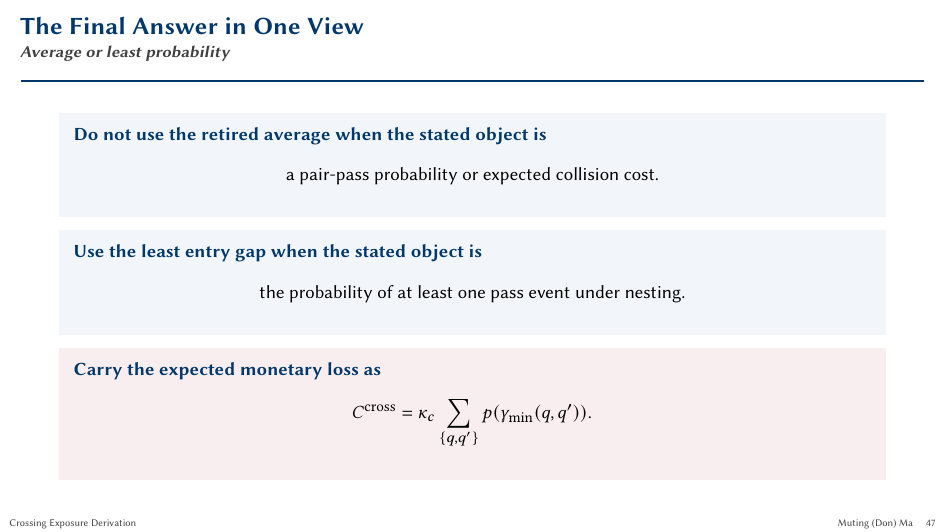
\includegraphics[width=0.58\textwidth]{../../BiObjectiveRevisionC1/Figures/ExpectedCollisionCost.png}}
  \caption{Adopted least-gap expected collision cost construction.}
  \label{fig:collision-cost}
\end{figure}

\updatehead{4}{Input needed from Dr. Gong}
\sumpara The requested input fixes the model and the order of the next evidence work. \sumparaend
\begin{tightitems}
  \item \fin Should the one-draw least-gap model remain the primary estimand while calibration is developed? \fine
  \item \fin Should the next work prioritize the audit and calibration package or practical-controller pilots? \fine
\end{tightitems}

\updatehead{5}{Before the next meeting}
\sumpara The deliverables address the nearest incomplete closure steps. \sumparaend
\begin{tightitems}
  \item \fin Export canonical pair records and the pair-level audit. \fine
  \item \fin Run the prescribed error-scale sensitivity. \fine
  \item \fin Specify controller comparisons and seed and demand pilots. \fine
\end{tightitems}

\vspace{0.25em}
{\footnotesize\textbf{Public artifacts:}
\artifact{https://github.com/mutingma123/OpenProjects/tree/main/BiObjectiveRevisionC1}{project folder};
\artifact{https://github.com/mutingma123/OpenProjects/tree/main/BiObjectiveRevisionC1/Figures}{selected snapshot}.\par}

\clearpage
\section{Stochastic Multiple Knapsack Manuscript}
\label{sec:knapsack}
\projectline{Stochastic Multiple Knapsack Manuscript}

\updatehead{1}{Current objective}
\sumpara The objective rebuilds the manuscript around a contribution supported by executable evidence. \sumparaend
\begin{tightitems}
  \item \fin Rebuild the stochastic multiple knapsack manuscript around a defensible contribution, a valid integer policy, and executable benchmarks. \fine
\end{tightitems}

\updatehead{2}{Progress since the last meeting}
\sumpara The progress combines the full manuscript dissection with the four-paper benchmark review. \sumparaend
\begin{tightitems}
  \item \fin \statusdone Built a 55-frame dissection with 62 logical slides that integrates all ten advisor points and every computational result. \fine
  \item \fin \statusdone Reviewed four close papers that separate human and stochastic evidence from structural and computational evidence \cite{gulmez2026,perreault2025,mancini2024,masmoudi2024}. \fine
  \item \fin \statusblocked The publication claim remains unsupported because the displayed feasibility proposition is false and the reported assignments come from the continuous relaxation. \fine
\end{tightitems}

\updatehead{3}{Key result or lesson}
\sumpara The key result narrows the contribution and identifies the concrete technical blockers. \sumparaend
\begin{tightitems}
  \item \fin The defensible core is a time-discounted two-stage formulation plus a continuous Benders proof of concept. \fine
  \item \fin Zero effort and zero completion contradict the current feasibility proposition, while 12 of 21 reported assignments are fractional. \fine
  \item \fin The \artifact{https://github.com/mutingma123/OpenProjects/blob/main/StochasticMultipleKnapsack/Figures/ManuscriptFinalVerdict.png}{public verdict} states the resulting revision boundary. \fine
\end{tightitems}

\begin{figure}[!ht]
  \centering
  \href{https://github.com/mutingma123/OpenProjects/blob/main/StochasticMultipleKnapsack/Figures/ManuscriptFinalVerdict.png}{%
    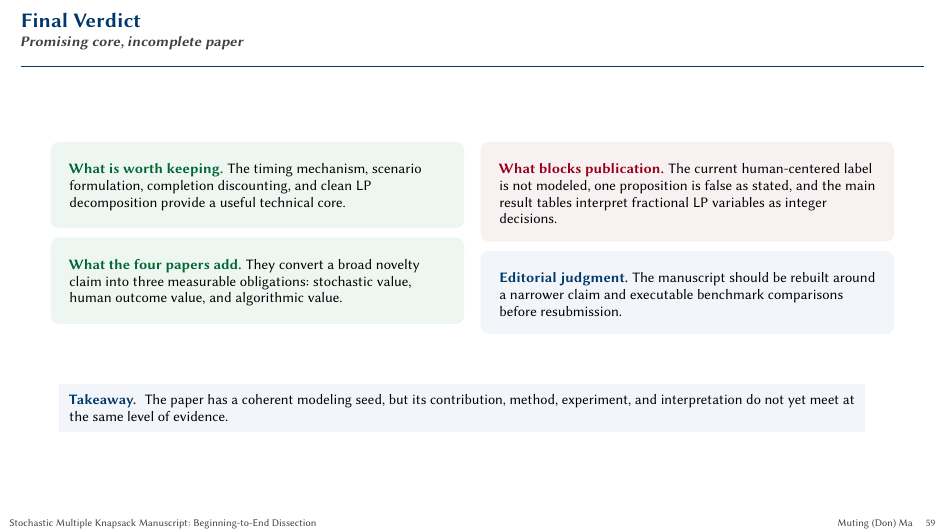
\includegraphics[width=0.58\textwidth]{../../StochasticMultipleKnapsack/Figures/ManuscriptFinalVerdict.png}}
  \caption{Current technical and editorial verdict.}
  \label{fig:knapsack-verdict}
\end{figure}

\updatehead{4}{Input needed from Dr. Gong}
\sumpara The requested input fixes the paper's identity and the integer solution route. \sumparaend
\begin{tightitems}
  \item \fin Should the paper narrow to managerial task scheduling or add an explicit individual outcome and fairness treatment? \fine
  \item \fin Should the first integer baseline use direct MILP, integer Benders, or rounding and repair? \fine
\end{tightitems}

\updatehead{5}{Before the next meeting}
\sumpara The deliverables repair the model before scaling the experiments. \sumparaend
\begin{tightitems}
  \item \fin Correct the proposition and prove nontriviality. \fine
  \item \fin Produce feasible integer incumbents and gaps. \fine
  \item \fin Prespecify held-out tests, seeds, scaling, and ablations. \fine
\end{tightitems}

\vspace{0.25em}
{\footnotesize\textbf{Public artifacts:}
\artifact{https://github.com/mutingma123/OpenProjects/tree/main/StochasticMultipleKnapsack}{project folder};
\artifact{https://github.com/mutingma123/OpenProjects/tree/main/StochasticMultipleKnapsack/Figures}{selected snapshot}.\par}

\clearpage
\phantomsection
\addcontentsline{toc}{section}{References}
\begin{thebibliography}{9}
\small

\bibitem{weller2026}
\fin O. Weller, M. Boratko, I. Naim, and J. Lee, ``On the Theoretical Limitations of Embedding-Based Retrieval,'' International Conference on Learning Representations, 2026. \fine
\href{https://openreview.net/forum?id=vNEY32I8Y8}{ICLR paper page}.

\bibitem{gulmez2026}
\fin E. G\"ulmez, M. E. Aydin, K. B. Urganci, S. C. Gamoura, and H. I. Koruca, ``Healthcare Staff Scheduling with Work-Life Balance Constraint Using Multi Objective Evolutionary Algorithms,'' \textit{Computers and Industrial Engineering}, vol. 220, 2026. \fine
\href{https://doi.org/10.1016/j.cie.2026.112287}{doi:10.1016/j.cie.2026.112287}.

\bibitem{perreault2025}
\fin C. Perreault-Lafleur, M. Carvalho, and G. Desaulniers, ``A Stochastic Integer Programming Approach to Reserve Staff Scheduling with Preferences,'' \textit{International Transactions in Operational Research}, vol. 32, no. 1, pp. 289 to 313, 2025. \fine
\href{https://doi.org/10.1111/itor.13298}{doi:10.1111/itor.13298}.

\bibitem{mancini2024}
\fin S. Mancini, C. Meloni, and M. Ciavotta, ``A Decomposition Approach for Multidimensional Knapsacks with Family-Split Penalties,'' \textit{International Transactions in Operational Research}, vol. 31, no. 4, pp. 2247 to 2271, 2024. \fine
\href{https://doi.org/10.1111/itor.13207}{doi:10.1111/itor.13207}.

\bibitem{masmoudi2024}
\fin M. Masmoudi, Y. Adouani, and B. Jarboui, ``LP Relaxation and Dynamic Programming Enhancing VNS for the Multiple Knapsack Problem with Setup,'' \textit{International Transactions in Operational Research}, vol. 31, no. 3, pp. 1890 to 1916, 2024. \fine
\href{https://doi.org/10.1111/itor.13213}{doi:10.1111/itor.13213}.

\end{thebibliography}

\end{document}
